\section{Présentation de mon projet de M2 }

Dans cette partie nous nous intéresserons à mon projet de deuxième année d'alternance que je commence à mener dès maintenant en parallèle de mes autres projets en cours. 

\subsection{Présentation}

Mon projet de M2 consiste à la réalisation d'un boitier compatible avec les rails DIN, intégrant un FPGA permettant d'effectuer diverses opérations de traitement. L'objetif fixé est de concevoir la carte PCB qui acceuillera les élements électroniques ainsi que la partie mécanique (le boitier). Ceci devra être fait en répondant à toutes les normes en vue d'une commercialisation sur le marché. 
\newline
L'objectif et aussi d'acquérir un savoir faire dans le but de décliner plusieurs modèles (avec des entrées/sorties et des dimensions variées) pour répondre à des exigences clients différentes.

\subsection {Pourquoi réaliser ce projet ? } 

L'interêt de la mise en oeuvre d'un tel boitier est de pouvoir répondre à un besoin client important. En effet ce boitier pouvant s'adapter sur un rail DIN pourra être utilisé pour réaliser des opérations (traitement vidéo, calculs spécifiques ..) que les autres équipements ne peuvent pas réaliser.

Par exemple dans le cas d'un automate qui possède une puissance de calculs limitée, les données seront transmises au boitier contenant le FPGA, traitées puis renvoyées dans l'automate. 

\subsection {Cahier des charges } 

Le projet doit répondre à un cahier des charges précis : 
\newline
\begin{itemize}
	\item Le boitier doit être compatible avec les rails DIN.
	\item La carte PCB doit être optimisée pour le boitier. Les contours de la carte seront établis en fonction de la forme du boitier.
	\item La carte électronique pourra être programmée par le biais d'un port USB.
	\item La carte électronique disposera de 4 connecteurs SFP qui pourront servir d'entrées ou de sortie.
	\item Le projet devra répondre au normes de comptatibilités électroniques.
	\item Le projet devra répondre au normes CE en vue d'une commercialisation. 

\end{itemize}


\subsection {Réalisation du boitier } 

Pour le momment,  j'ai commencé la réalisation du boitier qui acceuillera la carte pcb. Phoenix Contact est un fabriquant de solutions industrielles qui propose également un service de personnalisation de boitiers industriels. Ce service laisse un libre choix aux clients en ce qui concerne les types de boitiers souhaités, les dimensions du boitier ainsi que le choix des connecteurs utilisés.
\newline
Dans un premier temps, j'ai réalisé sur le site de Phoenix Contact un boitier compatible rail DIN répondant au exigences du cahier des charges. Une fois la configuration terminée, Phoenix Contact fournit le modèle 3D du boitier : 
\newpage
\begin{figure}[ht]
    \centering
    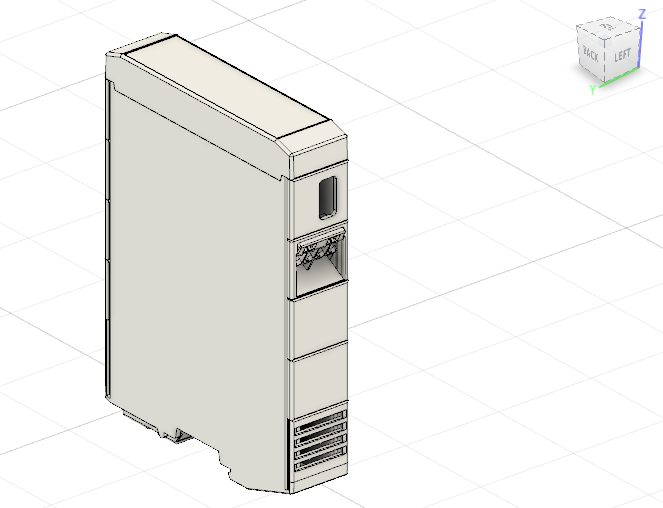
\includegraphics[scale=0.35]{img/boitier.PNG}
    \caption{Apperçu de la conception 3D du boitier }
    \label{fig:CameraCmdsettings}
\end{figure}

On peut également voir que les contours de la carte PCB sont eux aussi générés par le site web : 

\begin{figure}[ht]
    \centering
    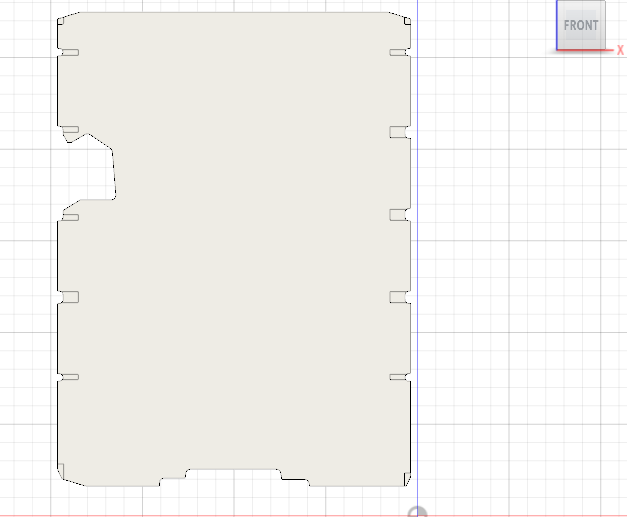
\includegraphics[scale=0.45]{img/pcb.PNG}
    \caption{Apperçu de la conception 3D du boitier }
    \label{fig:CameraCmdsettings}
\end{figure}

